As we said before, a Generative adversarial network are two different neural networks, the discriminator and the generator .The goal of the discriminator is to learn the correlation of the data in each of the frames,and the dependencies between them that comprise a real gait. Recurrent Neural Networks (RNNs) and Long Short Term Memory Networks (LSTMs) have shown considerable performance in this area. However, they have difficulties in handling the vanishing and the exploding gradient problems. The goal of the second neural network, the generator, that will generate movements of motion to this skeleton to create a walk. This neural network will send the results to the first network, and the goal would be for this generated motion to be classified as walking.

\pagebreak

 \begin{figure}[h]
	\centering
	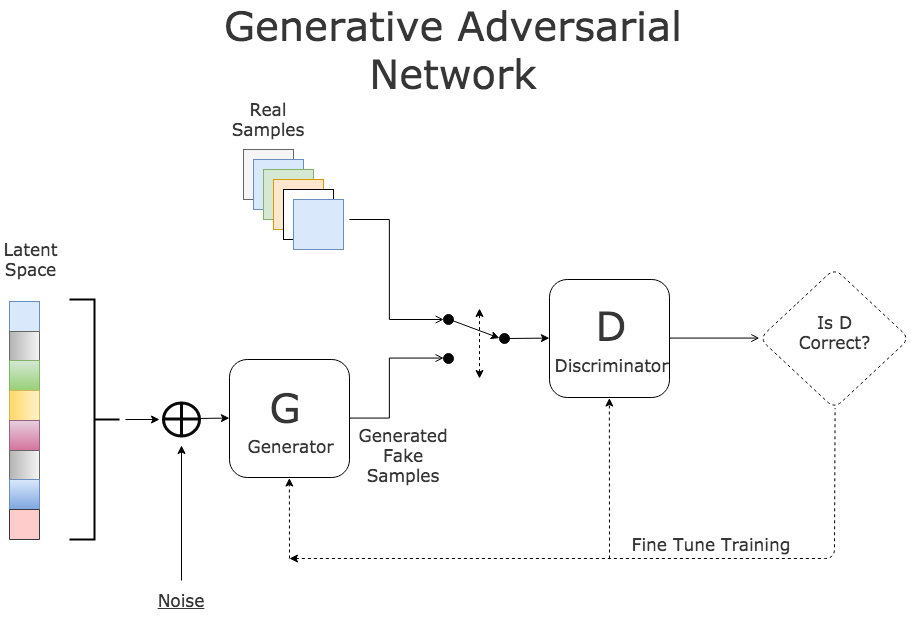
\includegraphics[width=0.8\textwidth]{figures/background/GAN.png}
	\captionsetup{labelformat=empty}
	\caption{\href{https://bolster.ai/blog/content/images/2020/04/GAN-1.png}
	{A simple GAN architecture}}
\end{figure}


In the initial phase, we sample some noise z using a normal or uniform distribution to the generator's input, and during the training the noise slowly is transforming to look like a sample from the training set. When the transformation exceed a threshold, then we assume that the generator created a sample that could be real. Therefore, the generator's task is to learn the distribution of input videos based on human actions, generate realistic samples, and fool a real/fake discriminator.\\

Subsequently, just consider that the GAN training as min-max game \cite{Human Action Generation with Generative Adversarial Networks}. A Mini-max game is domain of Game theory where two or more agents play a game against each other. These conflicting games both players try to find the Nash equilibrium of the game, which in GAN's case is a very hard to find. 

More specifically, given a data distribution $P_d$ whose p.d.f is $P_d$(x) where x $ \in R^d$, the aim of GAN is to train a neural network based generator G such that G(z)(s) fed by z ~ $P_z$ (i.e., the noise distribution) induce the generated distribution $P_g$ with the p.d.f $P_g$(x) coinciding the data distribution $P_d$ by minimizing the divergence between $P_g$ and $P_d$, which can be equivalently obtained via solving the following mini-max optimization problem:

$$min_Gmax_D (E_{P_d}[log(D(x))] + E_{P_z}[log (1 - D (G (z)))])$$

\noindent
where D is a neural-network based discriminator and for a given x and D (x) specifies the
probability x drawn from $P_d$ rather than $P_g$